% Describe RCPS Testbed & Testing Platform
% Describe evaluation metrics
% Describe testing scenarios and use cases
\chapter{Experimental Evaluation}
\label{chapter:evaluation}

Experimentally validating our timing analysis results is an important and necessary requirement. In order to obtain any level of confidence in our CPN-based work, the system design model needs to be completed implemented, and deployed on the target hardware platform. We have constructed a testbed \cite{kumarTestbed} to simulate and analyze resilient cyber-physical systems consisting of 32 Beaglebone Black development boards \cite{BBB}. We have chosen the light-weight ROS \cite{ROS} middleware layer and implemented our ROSMOD Component model \cite{kumarROSMOD} on top of it. This component model provides the same execution semantics and interaction patterns as our DREMS component model \cite{ISIS_F6_ISORC:13}. Our goal with this work is to (1) establish a set of distributed component-based applications, (2) translate this design model to our CPN analysis model, (3) deploy these applications on our testbed and accurately measure operation execution times, and finally (4) perform state space analysis on the generated CPN model to check for conservative results, compared against the real system execution.

\subsection{Challenges}

Experimental validation requires that online measurements of the real-time system match with the design-time timing analysis results in a way that the timing analysis results are always close but conservative. If the timing analysis results predict a deadline violation, this does not necessarily mean that the real system will violate deadlines but if the timing analysis and verification guarantees a lack of deadline violations, then the real system should follow this prediction. The design-time timing analysis primarily uses bounded state space analysis for such predictions. The analysis is bounded by necessity i.e. to tackle the state space explosion problem. Obtaining confidence from the timing analysis results depends entirely on the behavior of the system and the applied bounds. Recall that DREMS components are dormant by nature and need to be triggered either by timers or through interaction ports. Component-based applications using DREMS typically exhibit some periodic behavior i.e. sequences of interactions between components that repeats periodically. Each interaction sequence could involve a set of distributed components or assemblies. In such scenarios, design-time analysis bounds the state space generation to some constant multiple of the overall period of the application. The overall period here is some duration of time after which all of the sequences of interactions in the application have repetition. By analyzing some reasonably large multiple of the application period, the state space analysis both generates and searches a sufficiently large set of states of the system i.e. execution behaviors. Assuming the execution correctness of the timing analysis model and sufficiently conservative worst-case estimates of execution times, a complete absence of timing anomalies in this bounded state space is typically a good indication of a safely executing system. There are various ways to obtain the WCET values for individual operational steps but the easiest approach is to execute the design on our testbed and make accurate measurements.

%You also need to come up with a 'worst-case' input for the operation, as well as have to run a lot of experiments and compute the WCET from the data. 

WCET of component operational steps needs to be measured by having the component operation execute at highest priority with no other component threads intervening this process. Secondly, this experiment must be repeated multiple times with different inputs (if any), including the worst-case input. The worst-case measurement across multiple runs of the experiment gives us a \emph{pure execution time} of the code block. 

Obtaining the WCET values by this method is not only more realistic but also an accurate representation of the target system. Once these individual numbers are obtained, the values are plugged into the CPN through our business-logic models. Ideally, the CPN model, consisting of a composition of component operation models, when analyzed, produces results that closely resemble a real-system deployment of the component assembly. Such results would validate the modeling accuracy and the analysis results.

%Distributed CPS are hard to develop hardware/software for; because the software is coupled with the hardware and the physical system, software testing and deployment may be difficult - a problem only exacerbated by distributing the system.  These types of systems must be tested for performance assurances, reliability, and fail-safety.  Examples of these systems include UAV/UUV systems, fractionated satellite clusters, and networks of autonomous vehicles, all of which require strict guarantees about not only the performance of the system, but also the reliability of the system.  Because of the need for such strict design-time guarantees, many traditional techniques for software testing cannot be used.  Cloud-based software testing may not accurately reflect the performance of the software, since many of these systems use specialized embedded computers, and furthermore does not provide the capability to easily integrate a system simulation into the software testing loop.  For such systems, a closed-loop simulation testbed is necessary which can fully emulate the deployed system, including the physical characteristics of the nodes, the network characteristics of the systems, and the sensors and actuators used by the systems.

%Emerging industry standards and collaborations are progressing towards component-based system development and reuse, \emph{e.g.} AUTOSAR~\cite{autosar} in the automotive industry.  As these systems are becoming increasingly more reliant on collections of software components which must interact, they enable more advanced features, such as better safety or performance, but as a consequence require more thorough integration testing.  Comprehensive full systems integration is required for system analysis and deployment, and the development of relevant testing system architectures enables expedited iterative integration.  Developing these systems iteratively, by prototyping individual components and composing them can be expensive and time consuming, so tools and techniques are needed to expedite this process.  Our testbed architecture was developed to help address these issues and decrease the turn-around time for integration testing of distributed, resilient CPS.  

%Examples of such systems which can be prototyped and tested using this architecture are (1) autonomous cars, (2) controllers for continuous and discrete manufacturing plants, and (3) UAV swarms.  Each of these systems is characterized as a distributed CPS in which embedded controllers are networked to collectively control a system through cooperation.  Each subsystem or embedded computer senses and controls a specific aspect of the overall system and cooperates to achieve the overall system goal.  For instance, the autonomous car's subsystems of global navigation, pedestrian detection, lane detection, engine control, brake control, and steering control all must communicate and cooperate together to achieve full car autonomy.  The control algorithms for each of these subsystems must be tested with their sensors and actuators but also must be tested together with the rest of the systems.  It is these types of cooperating embedded controllers which are a distinguishing feature of distributed CPS.  Integration testing for these distributed CPS can be quickly and easily accomplished using hardware-in-the-loop simulation, but must accurately represent the real physical system, hardware, software, and network. 

%In scenarios like the automotive networked CPS, one of the main challenges with system testing is the discord between the standardized networking protocols and communication methods e.g. CAN bus, and the manufacturer-specific implementations of these methods. It is difficult to obtain public access to the implementation details for such interaction patterns and therefore pure simulation of the communication protocols using event-simulation tools  is not sufficient in validating resilient application performance. The comprehensive testing for such safety-critical systems require \emph{replicating the CPS} by using a testing infrastructure that provides similar hardware and executes the exact embedded control code that would execute on the final system. 

% Section on our RCPS Testbed
\section{Resilient Cyber-Physical Systems (RCPS) Testbed}

\subsection{Architecture}

The testbed consists of 32 \emph{RCPS nodes}, each of which is a Beaglebone Black (BBB) \cite{BBB} development board. We execute a full software stack including a ROS-based middleware, called ROSMOD \cite{kumarROSMOD} and the DREMS component model. For the subset of CPS we are interested in, the behavior of the CPS can be much more precisely emulated with these boards compared to running the applications inside of a standalone simulation. For example, NASA's CubeSat Launch Initiative (CSLI) \cite{CubeSat} provides opportunities for nanosatellites to be deployed into space for research. CubeSats are small (4-inch long) satellites running low-power embedded boards and being prepared for interplanetary missions \cite{CubeSat_Mars} to Mars. A distributed set of CubeSats can be easily tested with this architecture if it can be integrated with a high-fidelity space flight simulator.  

\begin{figure}[h]
    \centering
    \includegraphics[width=\textwidth]{rcps-architecture.png}
    \caption{Testbed Architecture}
    \label{fig:architecture}
\end{figure}

The Gigabit Ethernet port of each BBB is connected to a \emph{Communication Network} switch. This is a programmable OpenFlow \cite{openflow} switch, allowing users to program the flowtable of the switch to control the routes that packets follow and completely configure the full network and subnets required for their emulated deployment.  Furthermore, the configurability of the communications network enables per-link or per-flow bandwidth throttling, enabling precise network emulation.  The primary \emph{Development and Control} machine, running our software development tools, communicates with the BBBs using this network. After software applications are deployed on this testbed, the characteristics of the real CPS network can be enforced on the application network traffic. Therefore, this network emulates the physical network which a distributed CPS would experience on deployment.

Each RCPS node is also connected to a \emph{Physics Network} using a 10/100 USB-to-Ethernet adapter, since the BBBs only have one gigabit ethernet port. This network is connected to a \emph{Physics Simulation Machine} running Cyber-Physical Systems simulations. This network provides the infrastructure necessary to emulate CPS sensing and actuation in the loop, allowing application software to periodically receive sensor data and open interfaces to output actuator commands to the simulation.

The Physics Simulation Machine closes the interaction loop for the testbed nodes, allowing the physical dynamics of the RCPS nodes to be simulated in the environment in which it would be deployed, \emph{e.g.} satellites' orbital mechanics and interactions can be simulated for a satellite cluster in low Earth orbit (LEO). 

\section{ROSMOD Software Infrastructure}

The software infrastructure includes our model-driven toolsuite and DREMS-style component model called ROSMOD \cite{kumarROSMOD}, the Robot Operating System middleware \cite{ROS}, and component-based software applications developed for ROSMOD. The applications are cross-compiled for Beaglebone Black and the relevant processes are started at real-time priority with \emph{SCHED\_RR} linux real-time process scheduling using our ROSMOD deployment framework (Figure \ref{fig:workflow}).

\subsubsection{ROSMOD Modeling Language}

To enable the design, development, and testing of software on distributed CPS, we have developed a modeling language specific to the domain of distributed CPS which utilize ROS, the ROSMOD Modeling Language (RML). Figure \ref{fig:ROSMOD_Project} shows the metamodel for this language using GME \cite{Ledeczi01thegeneric} notation; the GME-based metamodel figure is very similar to a traditional UML class diagram with some minor differences in notation. RML captures all the relevant aspects of the sofware, the system (hardware and network), and the deployment which specifies how the software will be executed on the selected system.  Using ROSMOD, developers can create models which contain instances of the objects defined in RML. This approach of using a domain specific modeling language to define the semantics of the models allows us to check and enforce the models for correctness.  Furthermore, this approach allows us to develop generic utilities or extensions, called \emph{plugins} \cite{maroti2014next} which can act on any models created using ROSMOD, for instance generating and compiling the software automatically or automatically deploying and managing the software on the defined system. The rest of this section goes into the specific parts of the modeling language, called the metamodel, and how they define the entities in a ROSMOD Model.

\begin{figure*}[ht]
	\centering
	\includegraphics[width=\textwidth]{ROSMOD-Meta2.png}
	\caption{ROSMOD Metamodel.  Containment is specified from \emph{src} to \emph{dst} where the source has a containment attribute \emph{quantity}, meaning that \emph{quantity} objects of type \emph{src} can be contained in an object of type \emph{dst}. Pointers are specified as a one to one mapping from source to destination, using the name of the pointer. Sets allow for pointer containment. All objects contain a \emph{name} attribute of type \emph{string}, not shown for clarity.  Note: the metamodel is used to create the ROSMOD Modeling Language, but users do not see or interact with it; it is used to enforce proper model creation semantics.}
	\label{fig:ROSMOD_Project}	
\end{figure*}
\FloatBarrier

The top-level entity of RML is a \emph{Project}, which is shown in the upper left of Figure \ref{fig:ROSMOD_Project}.  The language supports a variety of modeling concepts that address structural and behavioral aspects for distributed embedded platforms. ROSMOD users can create models of software workspaces, required software libraries, embedded devices, network topologies, component constraints and hardware capabilities. The language also supports code development, particularly with regards to port interface implementations i.e. the execution code for operations owned and triggered by communication
ports or local timers. Below, we describe in detail the various aspects of this metamodel and how these concepts are integral to developing distributed CPS and rapid prototyping needs.

\subsubsection{Motivation for ROSMOD Software Model}

The goal of the ROSMOD software model is to provide a language to precisely model the application software. When using a DREMS-style component model, the software is primarily a collection of components, where each component is defined by its ports and timers. Building a precise model of the software has various benefits. Firstly, applying model-driven development techniques enables reuse of previously defined components i.e. a single component can be instantiated or copied or modified as required and executed on the runtime system. Secondly, the development time of the application can be reduced significantly as a large part of the runtime code can be fully generated based on templates. Lastly, a clear model of the software provides a canvas for design-time analysis. If the structural aspects of the software are captured in the model of the component assembly, and the behavioral properties of the components are encoded in the attributes of its ports and timers, then using translation rules, a design-time analysis model can be fully generated. 

\subsubsection{Software Model}

The \emph{Software} class in Figure \ref{fig:ROSMOD_Project} models a software workspace. A workspace, following ROS terminology, is a collection of applications that are developed and compiled together into binaries. Thus, each Software class can contain ROS applications, called \emph{Packages}, and \emph{Libraries} required for the applications. Packages consist of \emph{Messages}, \emph{Services} and \emph{Components}. Components contain a set of pointers to Libraries to establish dependence e.g. an \emph{ImageProcessor} component \emph{requires} OpenCV, an open-source computer vision library. Libraries are of two types: Source libraries and System libraries. Source libraries are standalone archives that can be retrieved, extracted and integrated into the software build system with no additional changes. System libraries are assumptions made by a software developer regarding the libraries pre-installed in the system. Here, system refers to the embedded device on which the component is intended to execute.

\emph{Messages} represent ROS message types used by publisher and subscriber ports for topic-based communication. Similarly, \emph{Services} describe the ROS peer-to-peer request-reply interaction pattern. Each service is characterized by a pair of messages, \emph{request} and \emph{response}. A client entity can call a service by sending a request message and awaiting a response. This interaction is presented to the user as a remote procedure call. Each ROSMOD component contains a finite set of communication ports. These ports refer to messages and services to concretize the communication interface. Components can also contain \emph{Timers} for time-triggered operation e.g. periodically sampling inertial measurement sensors while operating an unmanned aerial vehicle
(UAV).

\subsubsection{Motivation for ROSMOD System Model}

The goal of the ROSMOD system model is to provide a language to precisely model the network of computers capable of executing applications defined in the software model. The system model is necessary for both compilation and deployment. The software defined in the software model, and therefore the generated source code must be compiled down to a binary for runtime execution. An accurate model of the available runtime system provides necessary information for cross-compilation requirements and any integrated runtime load balancing features. The deployment framework can use the system model to find a suitable candidate device onto which the application processes are deployed. To automate this process, the system model must capture fine-grained details about each available device, including information such as the IP address, the user permissions, and means to access the device e.g. Secure Shell Protocol (SSH) \cite{ylonen2006secure}. As with the software model, this system model can be reused in all ROSMOD projects for a given hardware assembly, such as the RCPS tested. 

\subsubsection{System Model} 

A \emph{System Model} completely describes the hardware architecture of a system onto which the software can be deployed. A ROSMOD Project contains one or more \emph{Systems}. Each System contains one or more \emph{Hosts}, one or more \emph{Users}, one or more \emph{Networks}, and one or more \emph{Links}.  A host can contain one or more \emph{Network Interfaces}, which connect through a link to a network.  On this link the host's interface is assigned an IP address, which matches the subnet and netmask specification of the network. Additionally, a host has a set of references to users, which define the user-name, home directory, and ssh-key location for that user. The host itself has attributes which determine what kind of processor architecture it has, e.g. \emph{armv7l}, what operating system it is running, and lastly a combination of Device ID and Device ID Command which provide an additional means for specifying the type of host (and a way to determine it), for instance specifying the difference between a BeagleBone Black and an NVIDIA Jetson TK1 which both have armv7l architecture but can be separated by looking at the model name in the device tree.  Finally, a host may contain zero or more \emph{Capabilities} to which the component constraints (described in the previous section) are mapped.  The final relevant attribute is the \emph{Network Profile} attribute of a link. Using the network profile, which is specified as a time-series of bandwidth and latency values, we can configure the links of the network using the Linux TC to enforce time-varying bandwidth and latency. This network configuration is useful when running experiments on laboratory hardware for which the network is not representative of the deployed system's
network.

\subsubsection{Deployment and Experimentation}

\emph{Deployment} refers to the act of starting application processes on candidate hosts, where each host can provide for and satisfy all of the constraints of the processes e.g. general purpose input/output (GPIO) ports, CPU speed etc. Therefore, a deployment is a mapping between application processes and system hosts on which the application processes run. The ROSMOD Deployment Model makes this map a loose coupling to enable rapid testing and experimentation. Each Deployment consists of a set of \emph{Containers}. Each container, conceptually, is a set of processes that need to be
colocated. Containers also ensure that no process outside a container is deployed along with the container once it has been mapped to a host. Each container, therefore, contains a set of \emph{Nodes} (ROS terminology for processes). In each node, application developers instantiate one or more components previously defined in the Software model. Following the ROSMOD component model, each such instance maps to an executor thread that executes the operations in the component's operation queue.  Note that the same component can be instantiated multiple times even within the same node. Also note the container is not mapped to a specific host within the deployment model, but rather is automatically mapped to a host by the deployment infrastructure within an \emph{Experiment}.

As shown in Figure \ref{fig:ROSMOD_Project}, each project supports a set of \emph{Experiments}. Each experiment has pointers to one System model and one Deployment model. The system model provides the set of available devices and the deployment model provides the set of containers, where each container contains a set of component constraints that need satisfying (the union of all the container's nodes' component constraints). ROSMOD uses these sets to find a suitable mapping and then deploys the containers on the chosen host devices, if a mapping can be found which satisfies all the constraints of all the containers.  When the deployment infrastructure selects hosts from the system model for mapping, it first checks to see which of the system model's hosts are 1) reachable, 2) have valid login credentials, 3) have the correct architecture, operating system, and device ID, and 3) are not currently running any other compilation or experiment processes from any other user.  In the case that there are no available hosts in the system or the deployment's constraints cannot be satisfied, the infrastructure informs the user. Upon successful deployment of the experiment, the infrastructure automatically stores the specific mapping relevant to the deployed experiment for later management and destruction. When such experiments are stopped, ROSMOD retrieves the component logs from the hosts and displays results. 

Such a loose coupling between the deployment model and the system model, along with the infrastructure automatically mapping the containers to valid, unused hosts enables the execution of the same
deployment onto subsets of a large system, for instance running many instances of the same deployment as separate experiments in parallel on a large cluster of embedded devices.  Additionally such a loose coupling enables redeployment onto a completely different system by simply changing the experiment's system model reference; the infrastructure will automatically verify that the new system meets the constraints of the deployment and has available hosts.

\subsection{Deployment Infrastructure}
\label{sec:Deployment_Infrastructure}

The workflow for software deployment is as shown Figure \ref{fig:workflow}. After the user has generated and compiled the software model into binary executables, they can run an experiment that has valid deployment model and system model references. Every ROSMOD workspace is generated with an additional \emph{node} package. This builds a generic node executable that can dynamically load libraries. When the software infrastructure generates and compiles the source code for the software model, the components are compiled into dynamically loadable libraries, one for each component
definition along with a single executable corresponding to the generic node package. The first step the deployment infrastructure performs when running an experiment is generating the XML files which contain metadata about each ROS node modeled in the ROSMOD Deployment Model. This metadata includes the component instances in each node and the appropriate component libraries to be loaded. Based on the XML file supplied to the node executable, the node will behave as one of the ROS nodes in the deployment model. This allows for a reusable framework where a generic executable (1) loads an XML file, (2) identifies the component instances in the node, (3) finds the necessary component libraries to load and (4) spawns the executor threads bound to each component.

\begin{figure}[ht]
	\centering
	\includegraphics[width=\textwidth]{DeploymentInfrastructure.png}
	\caption{Software Deployment Workflow}
	\label{fig:workflow}
\end{figure}
\FloatBarrier

The reason for having the components be libraries that are loaded at run-time by a node executable is 1) to help enforce separation between each component's code, 2) to shorten the compilation time (which may be quite long for embedded processors and complex models), and most importantly 3) to enable the ability for users to change the mapping of component instances to processes without the need to recompile any of the code.  Because ROSMOD is focused on the rapid development and deployment of reusable software components, we designed the infrastructure to allow users to experiment with which components are collocated within processes dynamically and rapidly iterate through several scenarios and experiments without having to wait for code compilations between experiments.  Finally, such a component-based deployment framework enables unit testing and integration testing in a very well-defined manner for the software components.  If an error occurs during the execution of an application on a system, the user can easily and quickly break the deployment down into sub-deployments for unit-testing of only the relevant components to determine the source of the error.

In the above architecture, the deployment needs three primary ingredients: (1) the generic node executable, (2) dynamically loadable component libraries, and (3) an XML file for each ROS node in the
deployment model. For each new node added to the deployment model, by merely regenerating the XML files, we can establish a new deployment. The ROS workspace is rebuilt only if new component
definitions are added to the Software Model. This architecture not
only accelerates the development process but also ensures a separation
between the Software Model (i.e. the application structure) and
deployment-specific concerns e.g. component instantiation inside ROS
nodes.

When the user has selected an experiment to run, the deployment
infrastructure first determines whether the selected deployment can
execute on the selected system.  Like the software infrastructure
described above, the deployment infrastructure queries the selected
system to validate that the system is reachable, conforms to the
model, and has available hosts for deployment (i.e. they are not
currently running any compilation or deployment processes).  Once
those available hosts have been determined, the infrastructure
attempts to map the deployment's containers to the available hosts
based on the constraints and capabilities of the two sets.  If the
constraints cannot be satisfied by the capabilities of the available
hosts, the user is informed and the deployment of the experiment is
halted.  If the capabilities of the hosts do satisfy the constraints
of the containers and their associated components, the deployment
infrastructure generates the required XML files for the deployment and
copies the XML files and the binaries over to the selected hosts,
before starting the relevant processes.  Finally, if all of those
steps are successful, the infrastructure saves the mapping into the
model for user inspection and for later teardown of the experiment.

When the user chooses to end a currently running experiment, the
deployment infrastructure verifies that the experiment is still
running before stopping the associated processes, copying the relevant
log files back, cleaning up the deployment artifacts from the hosts,
and removing the saved experiment mapping from the model.

\section{Evaluation of Timing Analysis Results}

Experimental validation should demonstrate that online measurements of the real-time system match with the timing analysis results in a way that the timing analysis results are always close but conservative. The goal of the analysis is to obtain a fairly accurate estimation of the runtime behavior i.e. estimates of component timing behavior that isn't so conservative that the results are useless. If the real execution of a specific operation takes 100 milliseconds and the timing analysis is 135 milliseconds, then this is close but conservative. On the other hand, if the design-time analysis predicts the execution time to be in the order of seconds or tens of seconds, then the analysis is conservative but grossly over-estimate. One of the biggest assumptions in our CPN work is the knowledge of worst-case execution times of the individual steps in the component operations. We have previously designed \cite{SEUS} a business-logic modeling grammar that captures the temporal behavior of component operations, especially WCET metrics for the different code blocks inside an operation. For example, consider a simple client-server example as shown in Figure \ref{fig:rmi_application}. The client component is periodically triggered by an internal timer and executes a synchronous remote method invocation to a remote server component. The interaction here demands that the client component be blocked for the duration of time it takes the server to receive the operation, process its message queue, execute the relevant callback, and respond with output. 

Note that in Figure \ref{fig:rmi_application}, we only annotate isolated code blocks that take a fixed amount of execution time on a specific hardware architecture. These are the only measurements that we can reliably make with repeated testing and instrumentation. The client-side blocking delay is not measured because the number of factors responsible for this delay are numerous e.g. server's message queue state, scheduling non-determinism, network delays etc. In order to be able to predict this delay, we need to use state space analysis and search through the tree of possible executions to identify the worst-case blocking delay. This also means that our CPN model must capture and account for such delay-causing factors. 

The remainder of this section presents various primitive interaction patterns and assemblies that have been evaluated. The results are restricted to simple cases, though we have tested on medium-to-large scale examples spanning 25-30 computing nodes, and with up to a 100 components. The scalability of our model, however, is not within the scope of this paper as we have previously evaluated this metric \cite{SEUS}. As mentioned earlier, in all of our tests, we use the ROS \cite{ROS} middleware and our ROSMOD \cite{kumarROSMOD} component model. 

\subsection{Understanding the CPN Analysis Plots}

By performing state space analysis, we are analyzing a bounded tree of possible component behaviors. By identifying the worst-case execution trace in this tree, we're able to obtain a suitable conservative candidate execution that represents a possible behavior. Once this trace is identified, we plot the execution time behavior of all components in this trace. This pattern is followed in all of the following plots. Figure \ref{fig:understanding-the-plots} describes the analysis plots presented later in this chapter. Each subplot in this figure represents the execution of a component operation. The x axis of this plot represents the analysis time, and the y axis represents the execution time of the operation. Each execution is shown as a rectangular pulse, the amplitude of which is the execution time of the operation. The rising edge of the pulse represents the enqueue time stamp of the operation i.e. the time instant when a request for this operation was enqueued onto the component message queue. The falling edge of the pulse represents the completion time stamp i.e. the time instant when the component executor thread has completed execution of the operation and is ready to service the next request waiting in the queue. Since the execution time of the operation is calculated from the enqueue time instant, the plot can have intersecting pulses, as shown in the second subplot. Here a new operation request is enqueued onto the message queue while an existing instance of the operation request is being executed by the component executor thread. 

\begin{figure}[h]
	\centering
	\includegraphics[width=\textwidth]{understanding-the-plots}
	\caption{Interpreting Execution Time Plots}
	\label{fig:understanding-the-plots}
\end{figure}
\FloatBarrier


\subsection{Client-Server Interactions}

As shown in Figure \ref{fig:rmi_application}, a simple client server example involves a periodically triggered client component that fetches data from a remote server. Figure \ref{fig:client-server} shows our experimental trace of a simple distributed client-server sample. The client (client\_timer\_operation) is triggered every 500 ms, and performs floating-point calculations in a loop requiring the services of a remote operation.  %The loop bound is a random variable having a uniform distribution between some peak iteration count and 60\% of this peak. 
The server (Power\_operation) periodically receives this operation request and responds to it, taking about 1.2s to complete each operation instance. In this experiment, these component threads are running at high uninterrupted real-time priorities. 

\begin{figure}[h]
	\centering
	\includegraphics[width=\textwidth]{client-server}
	\caption{Experimental Observation: Client-Server Interactions}
	\label{fig:client-server}
\end{figure}
\FloatBarrier

Figure \ref{fig:client-server-cpn} shows the execution time plot derived from our CPN. As expected, since there are no other interruptions on the server side, the server is able to promptly respond to the client.

\begin{figure}[h]
	\centering
	\includegraphics[width=\textwidth]{client-server-cpn}
	\caption{CPN Analysis Results: Client-Server Interactions}
	\label{fig:client-server-cpn}
\end{figure}
\FloatBarrier

Table \ref{tbl:client-server} shows a summary of these results. Similar tables are included as part of all other experiments in this section. 

\begin{table}[]
\centering
\caption{Client Server Example - Summary of Results}
\label{tbl:client-server}
\begin{tabular}{|c|c|c|c|c|}
\hline
\textbf{\begin{tabular}[c]{@{}c@{}}Operation\\ Name\end{tabular}}  & \textbf{\begin{tabular}[c]{@{}c@{}}Component\\ Name\end{tabular}} & \textbf{\begin{tabular}[c]{@{}c@{}}Experimental \\ WCET (ms)\end{tabular}} & \textbf{\begin{tabular}[c]{@{}c@{}}Timing Analysis\\ WCET (ms)\end{tabular}} & \textbf{\begin{tabular}[c]{@{}c@{}}Deadline\\ (ms)\end{tabular}} \\ \hline
\begin{tabular}[c]{@{}c@{}}Power\\ Operation\end{tabular}          & Server                                                            & 829.155041                                                                                  & 852.0                                                                                                & 2000                                                             \\ \hline
\begin{tabular}[c]{@{}c@{}}Client\\ Timer\\ Operation\end{tabular} & Client                                                            & 1121.306376                                                                                 & 1152.0                                                                                               & 3000                                                             \\ \hline
\end{tabular}
\end{table}

\subsubsection{Bad Designs}

The goal of our CPN timing analysis is to identify bad component designs, unacceptable execution times, response times etc. There are various ways in which we can accidentally design a poorly performing client-server interaction. In the above case, the server operation takes 852 ms in its worst-case before responding to the client and unblocking the client executor thread. If instead, the server operation took 8.5 seconds, the client component will stay blocked for 10 times longer and the client timer expiries will not be serviced faster than the timer periods. This shows a simple use-case where the currently blocked client timer operation is starving subsequent timer expiries from being handled promptly. Figure \ref{fig:client-server-bad-case} shows our CPN predictions after simply changing this server execution time. 

\begin{figure}[h]
	\centering
	\includegraphics[width=\textwidth]{client-server-bad-case}
	\caption{CPN Analysis Results: Client-Server Response Times in Bad Designs}
	\label{fig:client-server-bad-case}
\end{figure}
\FloatBarrier

The execution time of the each new client-side timer operation is worse than the previous since the operation is spending much longer waiting in the queue. Recall that the execution time of a component operation includes the waiting time in the message queue. Even with a bounded state space that spans just 1 minute, it is clear that the client component message queue size is monotonically increasing. This is a use case where a client component execution is affected by delays caused on a remote server. Each client-server interaction delay will only be worsened when the server component has other operations to tend to aside from the client requests. 

\subsection{Publish-Subscribe Interactions}

Similar to the earlier example, consider the ROSMOD publish-subscribe interaction. A publisher is periodically triggered by a timer when this component broadcasts a message on a topic. A subscribing component receives this message and performs some computation. In this case, the timer period is set to 2 seconds i.e. every 2 seconds, these two component interact via publish-subscribe messaging passing. 

\begin{figure}[h]
	\centering
	\includegraphics[width=\textwidth]{publish-subscribe}
	\caption{Experimental Observation: Publish-Subscribe Interactions}
	\label{fig:publish-subscribe}
\end{figure}
\FloatBarrier

Figure \ref{fig:publish-subscribe} shows our testbed observations and Figure \ref{fig:publish-subscribe-cpn} shows our CPN analysis results. As evident, the CPN results closely match and validate this sample. Table \ref{tbl:publish_subscribe} summarizes the results.

\begin{figure}[h]
	\centering
	\includegraphics[width=\textwidth]{publish-subscribe-cpn}
	\caption{CPN Analysis Results: Publish-Subscribe Interactions}
	\label{fig:publish-subscribe-cpn}
\end{figure}
\FloatBarrier

\begin{table}[]
\centering
\caption{Publish Subscribe Example -- Summary of Results}
\label{tbl:publish_subscribe}
\begin{tabular}{|c|c|c|c|c|}
\hline
\textbf{\begin{tabular}[c]{@{}c@{}}Operation\\ Name\end{tabular}} & \textbf{\begin{tabular}[c]{@{}c@{}}Component\\ Name\end{tabular}} & \textbf{\begin{tabular}[c]{@{}c@{}}Experimental\\ WCET (ms)\end{tabular}} & \textbf{\begin{tabular}[c]{@{}c@{}}Timing Analysis\\ WCET (ms)\end{tabular}} & \textbf{\begin{tabular}[c]{@{}c@{}}Deadline\\ (ms)\end{tabular}} \\ \hline
\begin{tabular}[c]{@{}c@{}}Subscriber\\ Port\\ Operation\end{tabular} & Subscriber & 194.718958 & 200.0 & 1000 \\ \hline
\begin{tabular}[c]{@{}c@{}}Publisher\\ Timer\\ Operation\end{tabular} & Publisher & 249.2155 & 252.0 & 1000 \\ \hline
\end{tabular}
\end{table}

\subsubsection{Bad Designs}

Similar to the client-server example, we can explore another accidental bad design that may become hard to track. In a publish-subscribe interaction, the publisher and the subscriber are completely detached from each other i.e. delays in the subscriber operation do not affect the publisher. So, the only way the publisher component can affect its own behavior is how it is triggered. Periodically triggered data dissemination is the most commonly used streaming pattern aside from event-driven messaging. Here, if the period of the timer is decreased from 2 s to 10 ms, the publisher gets triggered too frequently and is seriously affected by a local design flaw.  

\begin{figure}[h]
	\centering
	\includegraphics[width=\textwidth]{publish-subscribe-bad-case}
	\caption{CPN Analysis Results: Time-triggered Publisher -- Periodicity Issues}
	\label{fig:publish-subscribe-bad-case}
\end{figure}
\FloatBarrier

Figure \ref{fig:publish-subscribe-bad-case} shows the CPN results for this design. The subscriber still performs as expected taking 200 ms to process each incoming message. But the publishing component is affected by the periodicity of its trigger. The publish\_timer fires every 10 ms, and at each expiry enqueues a timer operation request onto the publisher component's message queue. Each timer operation itself takes about 250 ms i.e. 25 times of the periodicity of its trigger. The inevitable result of this design is the monotonically rising execution times of each subsequent timer operation due to progressively delayed response. Here, the $t\_response\_time$ = $t\_dequeue$ - $t\_enqueue$ becomes progressively worse and eventually the publisher's message queue overflows. In the real experiment, we were unable to access the publisher component's device via remote shell as the device CPU was saturated. 

\subsection{Trajectory Planner}

In the past \cite{kumar2014colored}, we have used a \emph{Trajectory Planner} deployment to illustrate the utility of our state space analysis. As shown in Figure \ref{fig:trajectory-planner-components}, a Sensor component is periodically triggered every second by the \emph{sensor\_timer} at which point it publishes a notification to the Trajectory Planner, alerting the planner of new sensor state. The planner component receives this notification on its \emph{state\_subscriber}. On receiving this message, the planner executes a remote method invocation to the \emph{compute} server located in the Sensor, blocked and waiting for a response. At this point, the \emph{compute\_operation} is executed on the Sensor which returns the updated sensor state. This unblocks the planner component which uses the new sensor state to perform trajectory planning tasks. 

\begin{figure}[h]
	\centering
	\includegraphics[width=\textwidth]{trajectory-planner-components}
	\caption{Trajectory Planner Test}
	\label{fig:trajectory-planner-components}
\end{figure}
\FloatBarrier

Figure \ref{fig:trajectory-planner} shows the execution time plot of this sample where the sensor updates happen once a second. Figure \ref{fig:trajectory-planner-cpn} presents the CPN analysis plot and Table \ref{tbl:trajectory-planner} summarizes the results.

\begin{figure}[h]
	\centering
	\includegraphics[width=\textwidth]{trajectory-planner}
	\caption{Experimental Observation: Trajectory Planner}
	\label{fig:trajectory-planner}
\end{figure}
\FloatBarrier

This is a common interaction pattern in Cyber-Physical systems since embedded sensors are updated at a much higher frequency than a path planning entity. Thus, the planner can query the sensor at a lower rate to sample the sensor state. In this example, the planner is matching the frequency of the sensor since the execution cost is low. However, when more components are added to this deployment, the planner would have to fetch sensor state less frequently so as to not affect other system-level deadlines. 

\begin{figure}[h]
	\centering
	\includegraphics[width=\textwidth]{trajectory-planner-cpn}
	\caption{CPN Analysis Results: Trajectory Planner}
	\label{fig:trajectory-planner-cpn}
\end{figure}
\FloatBarrier

\begin{table}[]
	\centering
	\caption{Trajectory Planner Example -- Summary of Results}
	\label{tbl:trajectory-planner}
	\begin{tabular}{|c|c|c|c|c|}
		\hline
		\textbf{\begin{tabular}[c]{@{}c@{}}Operation\\ Name\end{tabular}} & \textbf{\begin{tabular}[c]{@{}c@{}}Component\\ Name\end{tabular}} & \textbf{\begin{tabular}[c]{@{}c@{}}Experimental\\ WCET (ms)\end{tabular}} & \textbf{\begin{tabular}[c]{@{}c@{}}Timing Analysis\\ WCET (ms)\end{tabular}} & \textbf{\begin{tabular}[c]{@{}c@{}}Deadline\\ (ms)\end{tabular}} \\ \hline
		\begin{tabular}[c]{@{}c@{}}Sensor\\ Timer\\ Operation\end{tabular} & Sensor & 199.00875 & 199.05 & 400 \\ \hline
		\begin{tabular}[c]{@{}c@{}}Compute\\ Operation\end{tabular} & Sensor & 445.373417 & 448.95 & 600 \\ \hline
		\begin{tabular}[c]{@{}c@{}}State\\ Subscriber\\ Operation\end{tabular} & \begin{tabular}[c]{@{}c@{}}Trajectory\\ Planner\end{tabular} & 446.874334 & 450.95 & 1000 \\ \hline
	\end{tabular}
\end{table}

If the sensor update frequency is increased to 100 ms, the sensor begins to notify the planner at a much higher frequency than expected. If there is no down-sampling on the planner's side, every single update will be handled by the planner, leading to dangerous queue size growth on the planner. Figure \ref{fig:trajectory-planner-bad-case} shows this deployment, as observed in the CPN analysis. 

\begin{figure}[h]
	\centering
	\includegraphics[width=\textwidth]{trajectory-planner-bad-case}
	\caption{CPN Analysis - Sensor firing too frequently}
	\label{fig:trajectory-planner-bad-case}
\end{figure}
\FloatBarrier

\subsection{Time-triggered Operations}

Time-triggered operations are an integral part of our component model. DREMS components are dormant by default. A timer has to trigger a inactive component for all subsequent interactions to happen. Since the DREMS component model supports various scheduling schemes on a single component message queue, this following test evaluates a priority first-in first-out (PFIFO) scheme. Multiple timers are created in a single component, each with a unique priority and period. A timer with a high frequency is assigned a high priority. Figure \ref{fig:periodic-timers} shows our experimental observations on a 5-timer example. 

Since ROSMOD components are associated with a single executor thread and component operations are also non-preemptive, a low-priority operation could theoretically run forever, starving a higher priority operation from ever executing, leading to deadline violations e.g. \emph{Timer\_1\_operation} can affect all other higher priority timers. Figure \ref{fig:periodic-timers-cpn} shows our CPN prediction where such a scenario is evident. It can be seen that \emph{Timer\_5\_operation}, the timer with the highest priority is periodically seeing spikes in execution time, courtesy of other lower priority operations consuming CPU without preemption. Table \ref{tbl:periodic-timers} summarizes the results.

\begin{figure}[h]
	\centering
	\includegraphics[width=\textwidth]{periodic-timers}
	\caption{Experimental Observation: Periodic Timers}
	\label{fig:periodic-timers}
\end{figure}
\FloatBarrier

\begin{figure}[h]
	\centering
	\includegraphics[width=\textwidth]{periodic-timers-cpn}
	\caption{CPN Analysis Results: Periodic Timers}
	\label{fig:periodic-timers-cpn}
\end{figure}
\FloatBarrier

\begin{table}[]
	\centering
	\caption{Periodic Timers -- Summary of Results}
	\label{tbl:periodic-timers}
	\begin{tabular}{|c|c|c|c|c|}
		\hline
		\textbf{\begin{tabular}[c]{@{}c@{}}Operation\\ Name\end{tabular}} & \textbf{\begin{tabular}[c]{@{}c@{}}Component\\ Name\end{tabular}} & \textbf{\begin{tabular}[c]{@{}c@{}}Experimental\\ WCET (ms)\end{tabular}} & \textbf{\begin{tabular}[c]{@{}c@{}}Timing Analysis\\ WCET (ms)\end{tabular}} & \textbf{\begin{tabular}[c]{@{}c@{}}Deadline\\ (ms)\end{tabular}} \\ \hline
		Timer\_1                                                          & Component\_1                                                      & 243.160041                                                                & 253.0                                                                        & 300                                                              \\ \hline
		Timer\_2                                                          & Component\_1                                                      & 122.4165                                                                  & 138.0                                                                        & 150                                                              \\ \hline
		Timer\_3                                                          & Component\_1                                                      & 62.789916                                                                 & 69.5                                                                         & 75                                                               \\ \hline
		Timer\_4                                                          & Component\_1                                                      & 28.962792                                                                 & 29.54                                                                        & 37.5                                                             \\ \hline
		Timer\_5                                                          & Component\_1                                                      & 5.15275                                                                   & 9.89                                                                         & 10                                                               \\ \hline
	\end{tabular}
\end{table}

\subsection{Long-Running Operations}
\label{sec:long_running_operations}

Our ROSMOD component model implements a non-preemptive component operation scheduling scheme. A component operation that is in the queue, regardless of its priority, must wait for the currently executing operation to run to completion. This is a strict rule for operation scheduling and does not work best in all system designs e.g. in a long-running computation-intensive application, rejuvenating the executing operation periodically and restarting it at a previous checkpoint increases the likelihood of successfully completing the application execution. In applications executing long-running artificial intelligence (AI) search algorithms e.g. flight path planning algorithms, the computation should not hinder the prompt response requirements of highly critical operation requests such as sudden maneuver changes. Our ROSMOD component model does not support the \emph{cancellation} of long-running component operations to service other highly critical operations waiting in the queue. With a few minor modifications to our scheduling schemes, long running operations can, however, be suspended if a higher priority waiting operation requires service. With these additions, we are able to model and analyze component-based systems that support long-running operations, with checkpoints, enabling the novel integration of AI-type algorithms into our design and analysis framework. 

\subsubsection{Challenges}

One of the primary challenges here is to identify the semantics of a long-running component operation i.e. the scenarios under which the component operations scheduler suspends a cooperating long-running operation in favor of some other operation waiting in the queue. If a long-running computation is modeled as a sequence of execution steps with bounded checkpoints, then the operation would execute one step at a time and suspend at such checkpoints if necessary. An important challenge here is accurately identifying the priority difference between the long-running operation and the waiting operation. If the long-running operation is one checkpoint away from completion e.g. 100-200 ms of execution time, then strictly following our suspension rules would not be the most prudent choice since this operation is almost complete. However, if the waiting operation is a critical one, then regardless of the state of the long-running operation, the executing operation must be suspended. Secondly, the modeled long-running computation semantics must be incorporated into our component model so that any analysis results obtained can be suitably validated. 

\begin{figure}[h]
	\centering
	\includegraphics[width=\textwidth]{lro-semantics}
	\caption{Long Running Operations - Timing Diagram}
	\label{fig:lro-semantics}
\end{figure}
\FloatBarrier

\subsubsection{Implementation and Results}

In each long-running operation, we, therefore, include a synchronous \emph{checkpoint step}, as shown in Figure \ref{fig:lro-semantics}. The only assumption we make about this long-running operation is the periodicity of these checkpoint steps i.e. we know how frequently a new checkpoint is reached and we assume that the search algorithm used by the long-running operation is capable of reaching a safe state (the checkpoint) before suspending itself if required. If a higher priority operation is ready and waiting in the queue, the long-running operation runs till the next checkpoint is reached, then suspends. The higher priority operation is then processed. Figure \ref{fig:three-components-lro-rosmod} shows the \emph{Software Model} for a component assembly with long running operations.

\begin{figure}[h]
	\centering
	\includegraphics[width=\textwidth]{three-components-lro-rosmod}
	\caption{Long Running Operation - Software Model}
	\label{fig:three-components-lro-rosmod}
\end{figure}
\FloatBarrier

The assembly consists of three components. Components \emph{Component\_1} and \emph{Component\_2} periodically publish on the \emph{ComponentName} message. \emph{Component\_3} periodically queries the server in \emph{Component\_2}. During these interactions, \emph{Component\_1} is performing a long running operation, the duration of which, is magnitudes larger than the average execution time of all other operations. Figure \ref{fig:three-components-lro} shows the execution time plot of this scenario, as measured on our testbed. 

\begin{figure}[h]
	\centering
	\includegraphics[width=\textwidth]{three-components-lro}
	\caption{Experimental Observation: Composed Component Assembly}
	\label{fig:three-components-lro}
\end{figure}
\FloatBarrier

For the CPN analysis, in order to obtain pure execution times of all these operations, each operation on each component is executed as a stand-alone function on the hardware. This way, we know the average and worst-case execution times of all operational steps with minimal interruptions. These numbers are injected into our generated CPN and state space analysis is performed. Figure \ref{fig:three-components-lro-cpn} shows our CPN analysis results for the same assembly.


\begin{figure}[h]
	\centering
	\includegraphics[width=\textwidth]{three-components-lro-cpn}
	\caption{CPN Analysis Results: Composed Component Assembly}
	\label{fig:three-components-lro-cpn}
\end{figure}
\FloatBarrier

\section{Analysis Limitations}

The business logic abstraction, as presented in Section \ref{sec:BL_Model}, is quite simple. This model represents abstractly how long the different blocks of code in an operation take, but does not fully model its behavior e.g. each non-blocking local code block is represented by a single WCET and no other properties. Since variables local to these functional code blocks are not modeled, this grammar also does not model conditional behavior. So, a high-level controller component that executes an event-driven state machine cannot be sufficiently modeled with the current model. Moreover, depending on the local state of such code blocks, different interaction patterns may be invoked e.g. if this high-level controller was responsible for performing periodic image processing to identify an object, the image processing (and all the associated image processing) would stop once the object was identified. Since this conditional interaction is not modeled in the CPN business logic grammar, the abstraction would assume that the image processing interactions always happen, instead of conditionally. Such abstractions can lead to gross over-estimation of the worst-case execution times of component operations. The primary reason for keeping the business logic grammar to this level of simplicity is to reduce the level of state space explosion i.e. modeling all local variables of an operation, and consequently the state changes for each of these variables would exponentially increase the size of the state space to be analyzed. Also, modeling the local variable state would also require (1) modeling the semantics of language with which the operation code was written, (2) evaluating all expressions using these local variables, and (3) calculating the result of all conditionals used in the business logic at all possible times. Such an analysis would be too refined, hard to implement and susceptible to semantic errors. 




\if 0
\subsection{Cyber-Physical Systems: Autonomous Ground Support Equipment (AGSE) Robot}

This section briefly describes an Autonomous Ground Support Equipment
(AGSE) robot that we designed, built, and deployed for the 2014-2015
NASA Student Launch Competition \cite{NASA_SL}. Special emphasis is
given to the value of a rapid system prototyping methodology in the
design process and how it allowed the AGSE to overcome many of the
challenges and problems encountered during the competition.  We also use
this example as our cyber-physical system for timing analysis.

The NASA Student Launch Initiative \cite{NASA_SL} is a research-based
competition partnered with NASA's Centennial Challenges, and aims to
stimulate rapid, low-cost development of rocket propulsion and space
exploration systems.  Both collegiate and non-academic teams
participate in the 8-month competition cycle composed of design,
fabrication, and testing of flight vehicles, payloads, and ground
support equipment.

The purpose of the 2014-2015 competition was to simulate a Mars Ascent
Vehicle (MAV) and to perform a sample recovery from the Martian
surface. The requirements for this simulation were twofold: (1) Design
and deploy a system termed the Autonomous Ground Support Equipment
(AGSE) that independently retrieves a sample off the ground and stores
it in the payload bay of a rocket, and (2) launch the rocket to an
altitude of 3000 ft. before safely recovering the sample.

The sample retrieval was accomplished using a robotic arm with
computer vision to find the sample and identify its orientation. After
successfully acquiring the sample, the system will then search for the
payload bay, identify its orientation, and place the sample within it.
The robot arm itself is a simple crane-style device akin to a
pick-and-place robot with a four-pronged gripper as the end effector.
It was designed to have a cylindrical workspace in order to most
efficiently access the ground around the system and rocket. It starts
in a known position and incrementally scans its workspace using a
built in camera. Image processing is performed to identify key
environmental features such as the sample and payload bay.  The
control flow in the AGSE software is shown in Figure
\ref{fig:AGSE-FlowChart}.

\begin{figure}[h]
	\centering
	\includegraphics[width=0.8\textwidth]{AGSE-FlowChart.png}
	\caption{AGSE Control Flow Chart}
	\label{fig:AGSE-FlowChart}
\end{figure}
\FloatBarrier

While the driving requirements of the competition were fixed, many of
the minor rules regarding AGSE performance, behavior, and safety
requirements evolved and were augmented throughout the course of the
competition. The volatile nature of these rules combined with the
short eight month duration of the build cycle precipitated the need
for rapidly adjustable design and fabrication processes. As such, an
iterative, modular, design-build-test approach was implemented in
order to concurrently develop as many components of the hardware and
software systems as possible. An initial AGSE prototype was
conceptualized from off-the-shelf components and the mechanical and
software systems were built in parallel, integrated, and tested. These
preliminary results were then used in future development to produce a
more ideal structure with greater positional accuracy and system
robustness.  Due to the modular nature of the system's design, it was
not necessary to immediately build a completely new second system, so
incremental improvements could be made on a specific subsystem (such
as the robot's gripper, any single degree of freedom, image
processing, motor control, etc.) as the design evolved.

\subsubsection{Distributed Deployment}

\begin{figure}[h]
	\centering
	\includegraphics[width=\textwidth]{AGSE_Deployment.png}
	\caption{AGSE Package Deployment}
	\label{fig:AGSE_Deployment}
\end{figure}
\FloatBarrier

The AGSE robot is controlled by a distributed set of embedded
controllers. Figure \ref{fig:AGSE_Deployment} shows the high-level
design for the deployment architecture. There are three embedded
devices, each with its own responsibilities.  The reasons for the use
of multiple embedded controllers cooperating was two-fold: 1) given
the design decision to fully automate the robot to search the
workspace for both the sample and the payload bay, we needed an
embedded processor capable of performing image-based object detection
and 2) given the design of the robot to search a workspace with the
given degrees of freedom, we needed an embedded processor with the
required available General Purpose Input/Output (GPIO) and Special
Function Input/Output (SFIO) pins. 

To meet the first requirement, we selected the NVIDIA Jetson TK1, which is an embedded ARM controller
with 4+1 ARM cores and 192 CUDA cores, that consumes 10 W or less.
We could not use the Jetson to meet the second requirement since it
does not support enough GPIO to control the linear actuators and
retrieve feedback from them.  Furthermore, it lacks SFIO for encoder
pulse decoding.  Therefore, a BeagleBone Black was selected for the
motor control interface board because it has specific hardware for
decoding quadrature encoded pulses (QEP) and enough available GPIO for
controlling the linear actuators and reading limit switches.

Since one of the secondary requirements of the competition governed
pause control and state feedback to the operator of the AGSE (during
the competition execution), a second BeagleBone Black was introduced
which served to provide mechanical safety switches for pausing the
AGSE, LED panels indicating the state of the AGSE, and a touchscreen
showing what the AGSE sees as it searches the workspace for the sample
and the payload bay.  This BeagleBone Black resides the User Interface
Panel (UIP).

The NVIDIA Jetson TK1 periodically fetches the latest webcam feed,
performs image processing and high-level path planning, and updates a
global state machine. The Beaglebone Black (BBB) mounted on top of the
robot performs power management, low-level motor control and feedback
processing. Lastly, the User Input Panel (UIP) houses a second
Beaglebone Black which reacts to user input through switches and
provides feedback through touchscreen display and LED panel
display. The UIP also responsible for keeping the user
informed about the real-time state of the AGSE and the current webcam
feed. Each of these controllers host multiple ROS nodes with ROSMOD
component executor threads periodically performing algorithmic
computations, calculating new robotic paths and communicating to
coordinate and maintain the AGSE state.

\subsubsection{Software Prototyping with ROSMOD}

\begin{figure}[h]
	\centering
	\includegraphics[width=\textwidth]{AGSE-Deployment.png}
	\caption{AGSE Component Assembly}
	\label{fig:AGSE}
\end{figure}
\FloatBarrier

The AGSE software was iteratively designed and rapid prototyped using
our ROSMOD tool suite. The Software Model consists of 8 components
spread across three ROS packages - motor control, high-level state
machine control and image processing. Each package is characterized by
its local set of messages, service and interacting components. Note
that just as in ROS, packages can share messages so that components
can subscribe/publish/provide/require messages/services from other
packages. Figure \ref{fig:AGSE} shows the component assembly and
wiring as per the design. The \emph{radialControl} and
\emph{verticalControl} components are responsible for radial and
vertical actuation of the AGSE respectively. The
\emph{rotationControl} component is capable of controlling three servo
motors: (1) the base rotation servo, (2) the gripper rotation servo,
and finally the (3) gripper position servo that opens and closes the
robot gripper. A \emph{Camera} component deployed on the NVIDIA Jetson
TK1 provides a direct interface to the camera. Using the
\emph{CaptureImage\_Server}, the \emph{ImageProcessor} component
receives a snapshot of the camera feed for periodic processing
needs. This feed is also used by the \emph{userDisplay} component to
display the feed on the user input panel, as shown in Figure
\ref{fig:AGSE_Deployment}. The user input panel is the primary
interface between the ROSMOD applications and the user. The
\emph{userDisplay} component provides information to the user and the
\emph{userInputControl} receives data from the user, specifically to
read the various control switches on the panel e.g. the pause, alarm,
and debug switches. Lastly, a \emph{HighLevelControl} component
orchestrates the high-level state transitions and controls the
operation of the robotic arm. These transitions include commands such
as \emph{find\_payload\_bay}, \emph{find\_sample},
\emph{move\_to\_target} etc., each of which publishes messages to
other components to propagate the motor control commands.

The ROSMOD code generators enabled generation of nearly 60\% (6,000+
lines) of the total built code. As mentioned before, much of this code
includes port initialization, build system files, callback skeletons,
etc. that usually take up a significant amount of development time. As
developers, we had to fill in the missing pieces - the business logic
of the callbacks, completing the component interaction loops. This
code includes architecture-specific control, e.g. GPIO and encoder
readings, LED and switch settings, camera image acquisition, and
high-level control.

The final AGSE used in the 2014-2015 NASA SLI competition is shown in
Figure~\ref{fig:competition_AGSE}.

\begin{figure}[h]
	\centering
	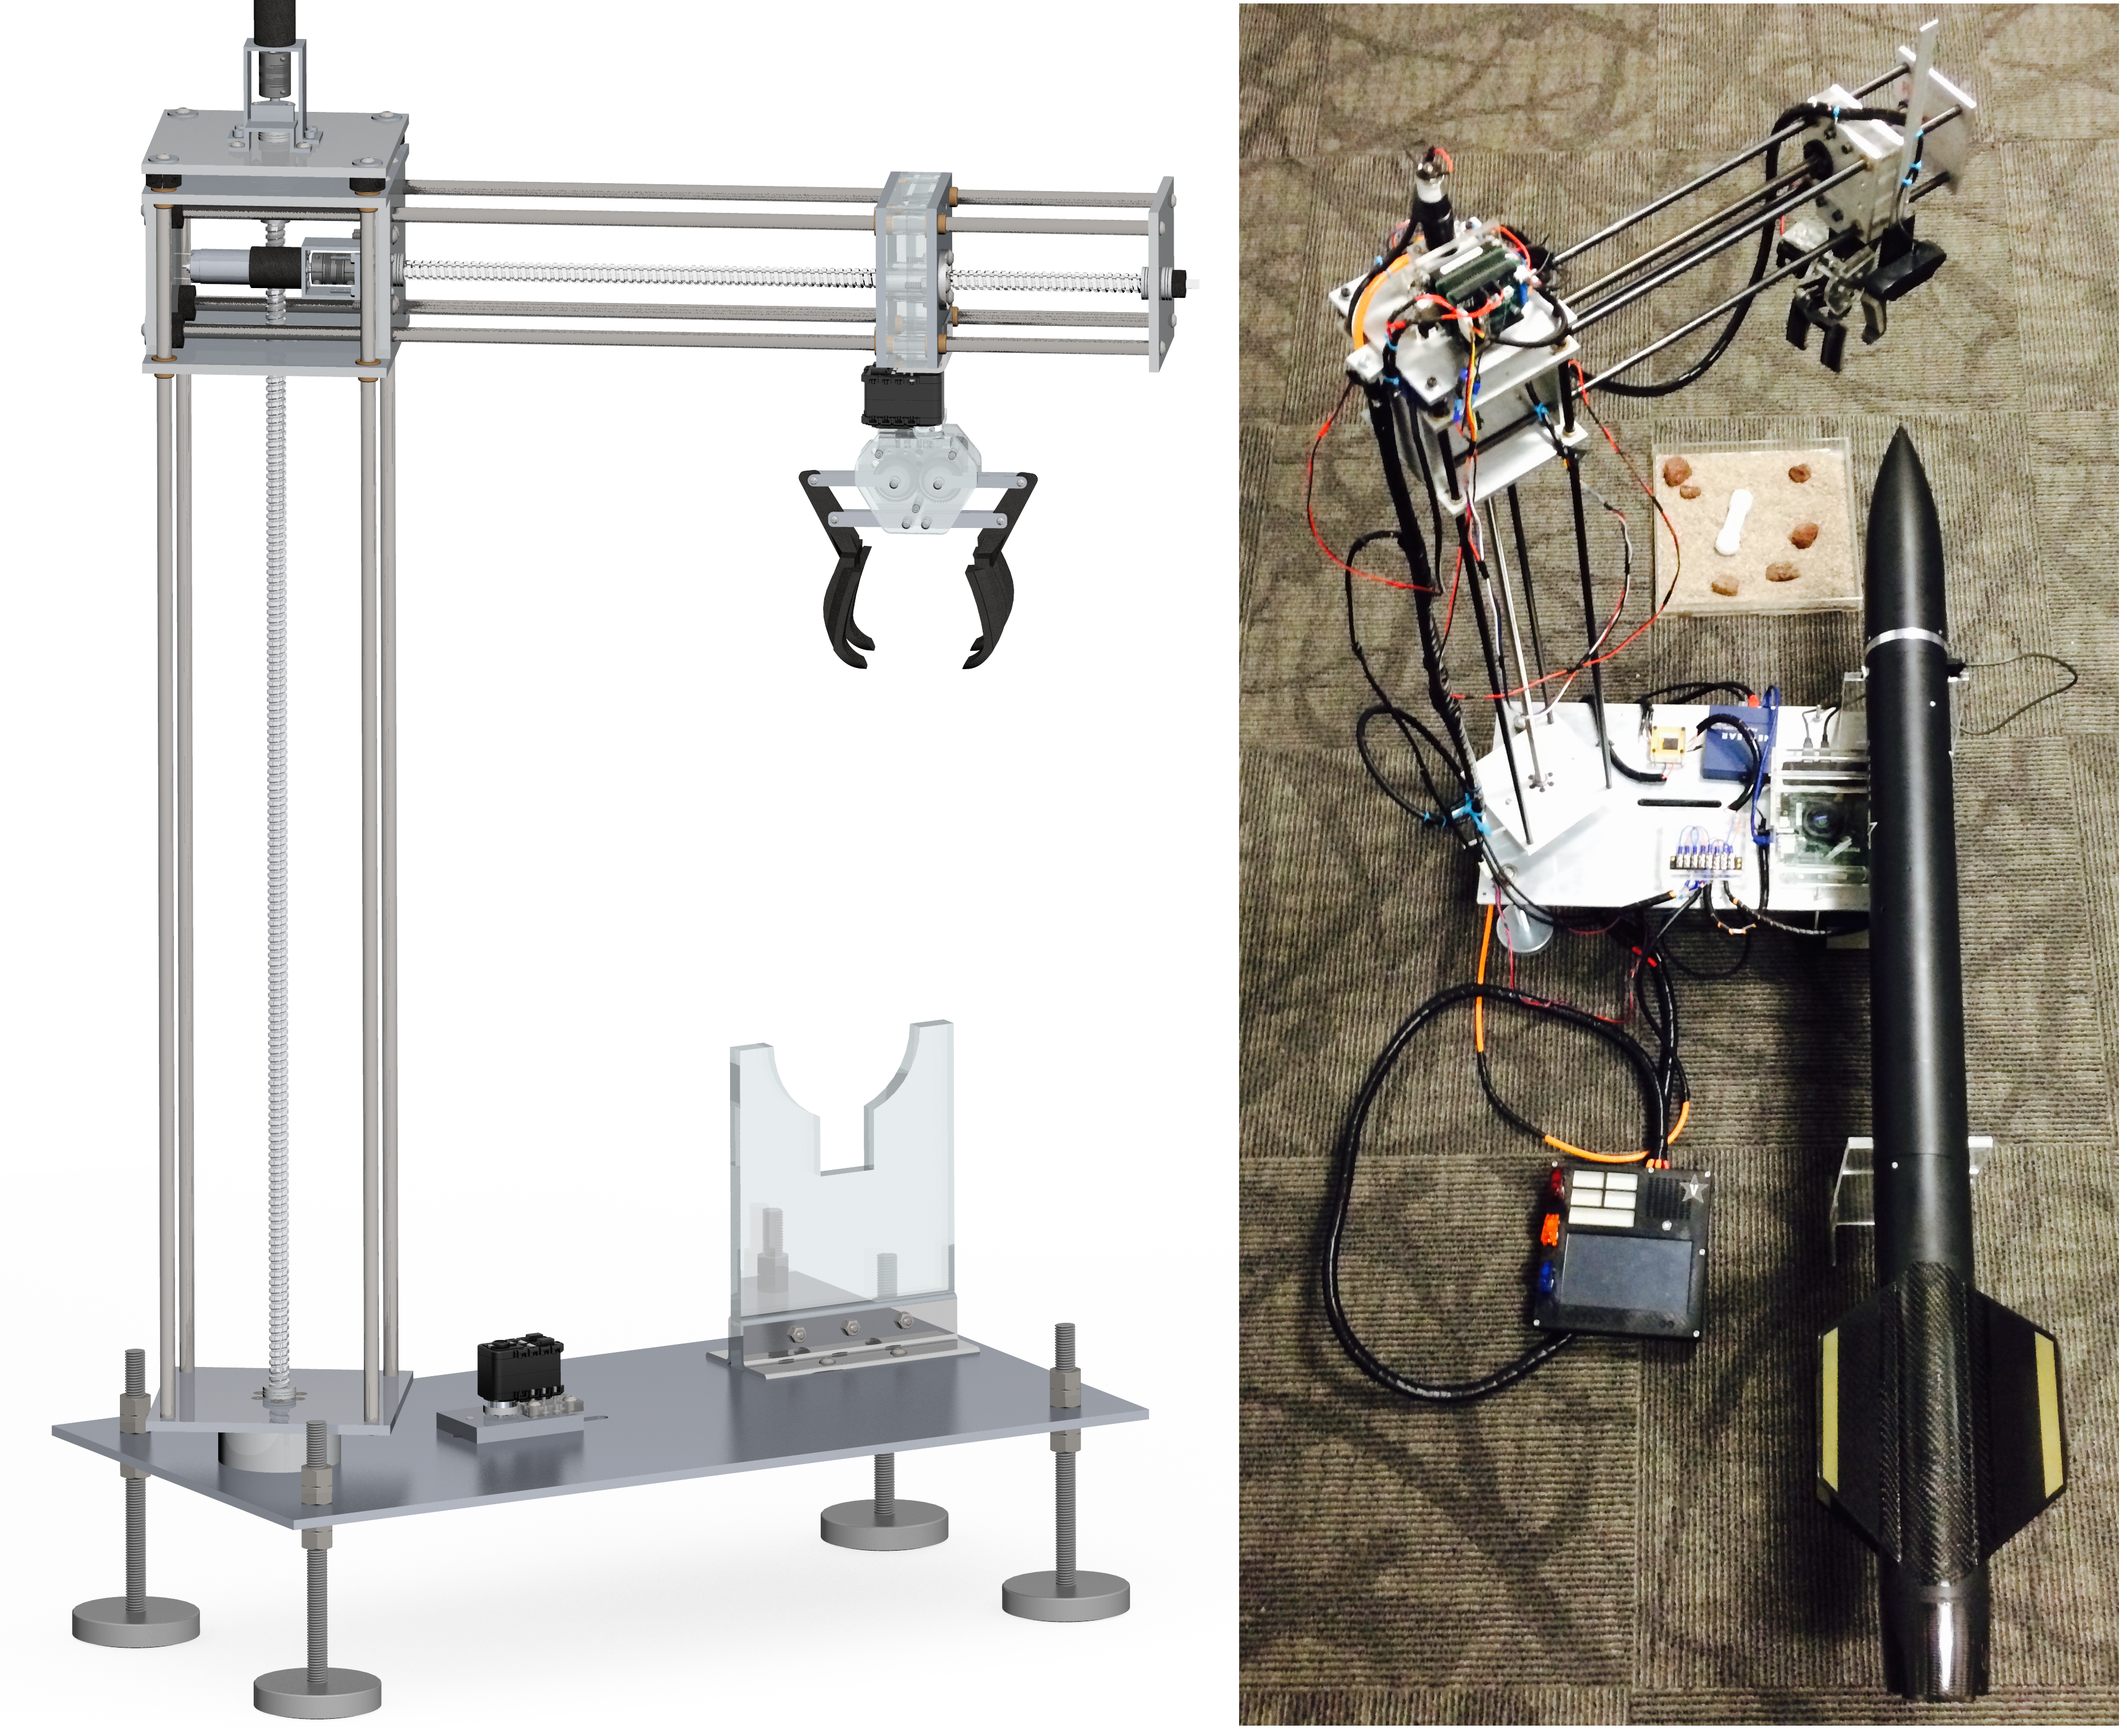
\includegraphics[width=\textwidth]{AGSE_Render.png}
	\caption{AGSE and rocket used in the 2014-2015 NASA SLI
		competition.  The UIP is shown in the bottom left of the
		picture, the Motor Control Board is on the top of the arm of
		the AGSE, and the NVIDIA Jetson is under the rocket.}
	\label{fig:competition_AGSE}
\end{figure}
\FloatBarrier

\subsubsection{Performance Assessment}

At the competition, the Vanderbilt AGSE was able to complete the
sample retrieval process in approximately $4.5$ minutes. The recovery
process, as shown in Figure \ref{fig:AGSE_Operation}, was successful,
with payload and rocket bay recognition occurring quickly and
efficiently. The AGSE was able to grasp the payload using only two of
its four padded end effector phalanges, and successfully deposited the
payload within the rocket bay. This operation received high marks from
the NASA officials and earned the competition's \emph{Autonomous
	Ground Support Equipment Award}.

\begin{figure}[t]
	\centering
	\includegraphics[width=\linewidth]{AGSE_Operation.png}
	\caption{AGSE Calibration and Testing}
	\label{fig:AGSE_Operation}	
\end{figure}
\FloatBarrier

System robustness was validated on the day of competition when a key
component failed and was able to be quickly replaced with a different
part with no detriment to system performance. The Dynamixel AX-12A
servo controlling the base rotational degree of freedom of the AGSE
suffered an irreparable failure of its gearbox and had to be removed
from the robot. A backup of the servo was not readily available, and a
different model servo by the same company had to be swapped in
instead.  This new model, a Dynamixel MX-28T, while having similar
performance as the old servo, had a different communication protocol
and mounting footprint, as well as a more complex control scheme.

The component-based nature of ROSMOD allowed quick modifications of
the business logic of the \emph{rotation\_controller} component to
update the system to use the new hardware.  The new control scheme was
quickly implemented and the control software was updated to account
for the new physical placement of the servo due to its different
mounting footprint. After these modifications were made, the AGSE was
able to perform at its optimal level during its part of the
competition.

\fi

